\documentclass[14pt,a4paper, oneside]{extreport}

%%%%%%%%%%%%%%%%%%%%%%%% Шрифты %%%%%%%%%%%%%%%%%%%%%%%%%%%%%%%%%
\usepackage{fontspec}         % пакет для подгрузки шрифтов
\setmainfont{Arial}   % задаёт основной шрифт документа

% Команда, которая нужна для корректного отображения длинных тире и некоторых других символов.
\defaultfontfeatures{Mapping=tex-text}

% why do we need \newfontfamily:
% http://tex.stackexchange.com/questions/91507/
\newfontfamily{\cyrillicfonttt}{Arial}
\newfontfamily{\cyrillicfont}{Arial}
\newfontfamily{\cyrillicfontsf}{Arial}

\usepackage{polyglossia}      % Пакет, который позволяет подгружать русские буквы
\setdefaultlanguage{russian}  % Основной язык документа
\setotherlanguage{english}    % Второстепенный язык документа
% Разные мелочи для русского языка из пакета babel
\setkeys{russian}{babelshorthands=true}


%%%%%%%%%% Работа с картинками %%%%%%%%%
\usepackage{graphicx}                  % Для вставки рисунков
\usepackage{graphics}

\usepackage{hyperref}
\hypersetup{
    unicode=true,           % позволяет использовать юникодные символы
    colorlinks=true,       	% true - цветные ссылки, false - ссылки в рамках
    urlcolor=blue,          % цвет ссылки на url
    linkcolor=red,          % внутренние ссылки
    citecolor=green,        % на библиографию
	pdfnewwindow=true,      % при щелчке в pdf на ссылку откроется новый pdf
	breaklinks              % если ссылка не умещается в одну строку, разбивать ли ее на две части?
}

\usepackage{csquotes}            % Еще инструменты для ссылок

%%%% Оформление %%%%%%%
\usepackage{extsizes} % Возможность сделать 14-й шрифт

% размер листа бумаги
\usepackage[paper=a4paper,top=10mm, bottom=10mm,left=35mm,right=35mm,includefoot,includehead]{geometry}

\usepackage{setspace}
\setlength{\parindent}{0mm} % Красная строка.
\setstretch{1.3}  % Межстрочный интервал
\setlength{\parskip}{4mm}   % Расстояние между абзацами
% Разные длины в латехе https://en.wikibooks.org/wiki/LaTeX/Lengths

\flushbottom                            % Эта команда заставляет LaTeX чуть растягивать строки, чтобы получить идеально прямоугольную страницу
\righthyphenmin=2                       % Разрешение переноса двух и более символов
\widowpenalty=300                     % Небольшое наказание за вдовствующую строку (одна строка абзаца на этой странице, остальное --- на следующей)
\clubpenalty=3000                     % Приличное наказание за сиротствующую строку (омерзительно висящая одинокая строка в начале страницы)
\tolerance=1000     % Ещё какое-то наказание.


\usepackage{fancyhdr} % Колонтитулы
\pagestyle{fancy}
	\rhead{\thepage}
	\cfoot{\footnotesize Школа Чародейства и Волшебства «Хогвартс»}

\renewcommand{\headrulewidth}{0.2pt}  % Толщина линий, отчеркивающих верхний
\renewcommand{\footrulewidth}{0.2pt}  % и нижний колонтитулы



%%% Редактирование заголовков
\usepackage{titlesec}  

% Убирает чеканутые отступы перед главами 
\titlespacing{\chapter}{0pt}{-20pt}{15pt} 

\usepackage{afterpage}  % Пакет, который позволяет настраивать параметры отдельной страницы

\usepackage[toc,page]{appendix} 
\usepackage{babel}


\begin{document}

% Всё, что идёт в окружении ниже устанавливается только для титульного листа! Это на всякий случай...

\begin{center}

\includegraphics[height=6cm]{hg.jpg}
\end{center}

\vspace{1cm}

{\fontsize{12}{1}\selectfont Мистеру Сергею Белоусову}

\vspace{2.5cm}
Мы рады проинформировать Вас, что Вам предоставлено место в Школе чародейства и волшебства «Хогвартс».

Пожалуйста, ознакомьтесь с приложенным к данному письму списком необходимых книг и предметов.

Занятия начинаются 1 сентября. Ждем вашу сову не позднее 31 июля.

Искренне ваша,

{\Large\fontspec{Carolina}{M. McGonagall}}

Минерва МакГонагалл

Заместитель директора

\vfill
\begin{center}
{\fontsize{12}{1}\selectfont \href{http://www.hogwartsishere.com/}{Сайт Школы}}

{\footnotesize Директор: Альбус Дамблдор

(Кавалер ордена Мерлина первой степени, основатель Ордена Феникса,председатель Международной Конфедерации Магов)}
\end{center}


%%%%%%%%%%%%%%%%%%% ОГЛАВЛЕНИЕ %%%%%%%%%%%%%%%%%%%%%%%%%%%%%%%%%%%%%%
\newpage
\newpage
\appendix
\renewcommand{\thesection}{\appendixname~\Asbuk{section}}

\section{Список необходмых книг и предметов}

\newcommand*{\mwand}{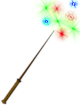
\includegraphics[scale=0.2]{wand.png}}
\renewcommand{\labelitemi}{\mwand}

\begin{itemize}
\item Волшебная палочка
\item Мантия-невидимка
\item Камень, оживляющий мёртвых
\item Задачник Демидовича
\end{itemize}

\newpage
\section{Список изучаемых предметов}

\begin{itemize}
\item Трансфигурация
\item История магии
\item Математический анализ
\end{itemize}

\end{document}